\section{Applications and Usage of Fog Computing}

\begin{figure}[H]
    \centering
    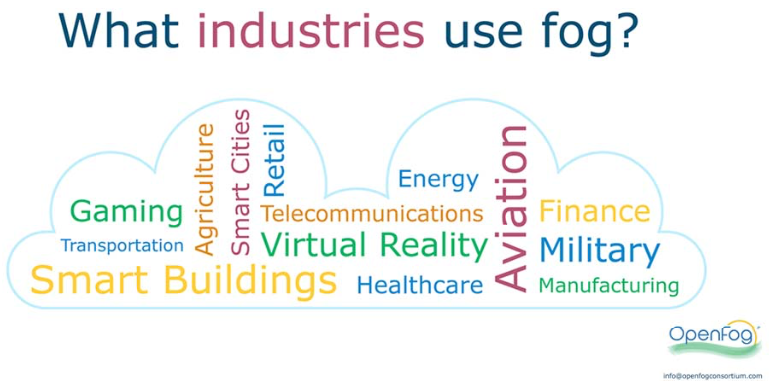
\includegraphics[width=.5\linewidth]{image/Applications of fog computing.png}
    \caption{Applications of fog computing}
    \caption*{img src: \cite{mukherjee2018survey}}
    \label{fig:applications of fog computing}
\end{figure}

Fog computing is the best approach to support geographically distributed, latency-sensitive, and QoS-aware IoT applications. It has a huge potential to meet the requirements of various applications like smart cities, healthcare, agriculture, aviation, energy, finance, gaming, manufacturing, military, retail, smart building, telecommunications, transportation, and virtual reality \cite{mukherjee2018survey}. Some are discussed below.

%-----------------------------------------------------------------subsection1

\subsection{Smart cities}

The major challenge of smart cities is the increased data demand and the number of IoT devices connected to the network. It is really hard to manage and keep track of the data generated. And also transferring this vast data between cloud and DCs causes delay, and effects communication costs \cite{sandra}. \par

Using fog computing, the amount of data sent to the cloud for processing can be reduced. This improves efficiency. There are many advantages by using fog computing for smart cities \cite{sandra}. \par

\begin{itemize}
    \item A minimal amount of data is sent to the cloud:  Instead of sending all the data to the cloud, fog manages the amount of data to be sent to the cloud. All the devices connected to the network generate a huge amount of data \cite{sandra}. And fog manages this data by performing data analysis operations \cite{webpage} like data filtering and trimming in the preprocessing layer \cite{mukherjee2018survey}, \cite{sandra}. Data is analyzed before sending it to the cloud so that unwanted data can be removed  and necessary data can be preserved \cite{webpage}, \cite{sandra}.
    \item Low latency: Fog nodes are capable of processing the data instead of sending it to the cloud. This saves the time of data being sent to the cloud and waiting for the response \cite{sandra}. As fog nodes are geographically much closer to the EUs than DCs, it is appropriate for latency-sensitive, and time-sensitive requests \cite{mukherjee2018survey}.
    \item Reduced bandwidth: Processing and transferring the data over the network demands high bandwidth. As data is distributed between the end devices in the fog it reduces the bandwidth consumption \cite{sandra}. 
    \item Better security: Data security is very important in any application, as sensitive and confidential data will be sent over the communication channels \cite{sandra}. Fog ensures better security with privacy, attestation, cryptographic techniques, and so on \cite{youtube}.
\end{itemize}

According to \cite{sandra}, smart cities is the best area to implement fog computing. As millions of things in the city are connected across the network they produce heterogeneous data of different aspects like air quality, public safety, road traffic, surveillance, waste management, and so on. Fog computing makes sure that all the data generated is managed and processed effectively \cite{sandra}. Some of the aspects are discussed below.

\begin{itemize}
    \item Traffic control: Different kinds of sensors are used to monitor and control traffic. Sensors can detect pedestrians, bikers, and drivers by measuring their speed of motion and the relative distance between them. The data collected in real-time is analyzed and decisions were made accordingly. For e.g. changing the colour of traffic lights \cite{sandra}. And video camera which can detect the flashlight of emergency services vehicles like ambulance, and fire trucks and changes the lights to clear the roads \cite{waheetha2016fog}.
    \item Waste management: This process requires a lot of time, money, and resources. Traditionally, each city will its have own schedule for garbage collection. Every household in the city keeps its bins outside for garbage collection on a specific day as mentioned in the schedule. Some bins will be empty and some overfilled. This results in a waste of resources and manpower as every household don't have an equal amount of waste. And some people might forget or will be unaware of garbage collection even though they have huge waste to be disposed of. And they should wait for the next possible day of garbage collection. The integration of sensors and fog computing supports real-time monitoring of garbage. By installing sensors in garbage bins they will notify users to change the bin if it's full. And by collecting all the garbage data of the whole city schedules can be optimized \cite{sandra}.
    \item Surveillance: Surveillance systems generate a huge amount of data. As fog nodes are closer to the EUs they capture and process the data quickly. The low latency feature of fog provides effective surveillance. This helps to detect violence in public places in real-time and situations where security, police, and fire services are necessary \cite{sandra}.
\end{itemize}

%-----------------------------------------------------------------subsection2

\subsection{Healthcare}

The main idea behind healthcare IoT is to make it easier for patients to consult their doctors anytime, anywhere possible. But the healthcare system encounters some challenges like processing of big data, the geographic distribution of users, privacy and security. So, fog computing is the best approach for healthcare IoT \cite{jennifer}. \par

As mentioned above fog is capable of processing big data by performing data analysis operations \cite{webpage} and fog nodes can process data instead of sending it to the cloud \cite{sandra}. Fog ensures privacy and security with predefined authorization techniques and exposes data through a secured channel. Only an authorized person can hold the data and make changes to it. Instead of sending health records every time, users can provide access to doctors, pharmacies, and other healthcare personnel so that they can have a real-time update of the user's condition \cite{jennifer}. \par

Sensor installed devices can be used as wearables to monitor patient's condition e.g. blood pressure, heart rate, and many more. These smart devices can also remind users about their physical activity. These are life savior for elderly people who live alone. Any change in the patient's condition alerts the doctor and people related to him/her. Data collected from these devices helps a doctor to monitor patients from time to time. And, sensor installed devices can also be used to track the location of the medical equipment in hospitals like wheelchairs, oxygen pumps, stretchers, and so on. Besides, sensor installed devices can also be used to monitor temperature, and humidity \cite{dr}. 

Healthcare IoT using fog computing reduces costs as one can monitor the patient's condition in real-time. No unnecessary visits to the hospitals which saves time and resources. Continuous monitoring helps doctors to diagnose patient's problems earlier \cite{dr}. 